 \chapter{Architektur}
In diesem Kapitel wird die Software Architektur erarbeitet.  
Es soll sowohl die Problemdomäne abstrakt mittels Domänenmodell analysiert werden, als auch ein Klassendesign mittels Schichtendiagramm erarbeitet werden.

\section{Übersicht}
Die Applikation hat eine typische 3-Tier Architektur. Auf der Clientseite wird die Single Page Application im Webbrowser ausgeführt. Die Serverseite handelt die Daten und stellt sie der Clientseite zur Verfügung. Die Daten werden auf einer Datenbank persistiert.
\begin{figure}[H]
\center
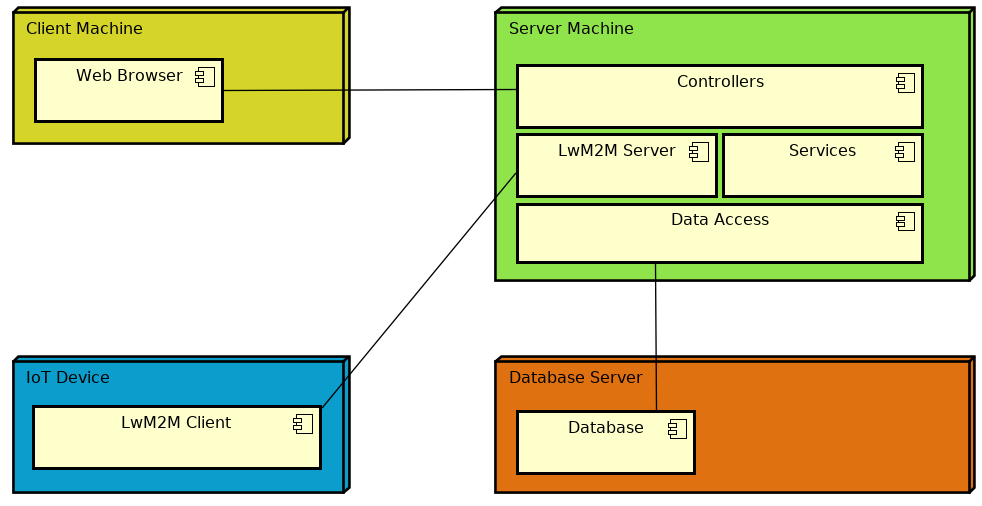
\includegraphics[scale=0.6]{images/architekturuebersicht}\caption{Architekturübersicht}
\end{figure}
\subsubsection{Client}
Die Clientseite wird als Single Page Application implementiert. Die Trennung zwischen Darstellung und Daten kann somit optimal vollzogen werden. Die Single-Page Applikation wird mittels dem evaluierten Aurelia Framework implementiert. Aurelia stellt die vom Server zur Verfügung gestellten Daten dar und ist zuständig für die Benutzerinteraktion und das Nachladen von neuen Daten. Da die MVC Komponenten sich beim Client befinden, wird ein häufiges Nachladen und serverseitiges Rendering verhindert. Dies hilft, um die Applikation auch bei mehreren Usern performant zu halten.
\subsubsection{Server}
Das Back-End wird als JEE Server realisiert. Das Spring MVC Framework soll die Entwicklung vereinfachen. Die Serverkomponente ist für die Bereitstellung der Daten an den Client verantwortlich. Dafür muss sie die Kommunikation zu den IoT Devices sicherstellen um zum einen die gewünschten Informationen zu erhalten und zum anderen um weitere Aktionen gemäss Use Cases durchzuführen. Die Daten sollen über ein REST API den Clients zu Verfügung gestellt werden.
\subsubsection{IoT Device}
Das IoT Device stellt über einen Kommunikationsendpunkt Daten zur Vefügung. Sowohl das Kommunikationsprotokoll, als auch die Form der Daten können variieren. IoT Devices kommunizieren mit dem Management Server und niemals direkt mit den Clients.
\subsubsection{Datenbank}
Als Datenbank wurde MongoDB evaluiert. Die Datenbank kann entweder auf dem gleichen-, oder auf einem entfernten physischen Rechner gestartet werden. Die Datenbank persistiert die Informationen zu den managed Devices.
\newpage


\begin{landscape}
\section{Klassenstruktur}
\subsection{Klassendiagramm}
\begin{figure}[H]
\centering
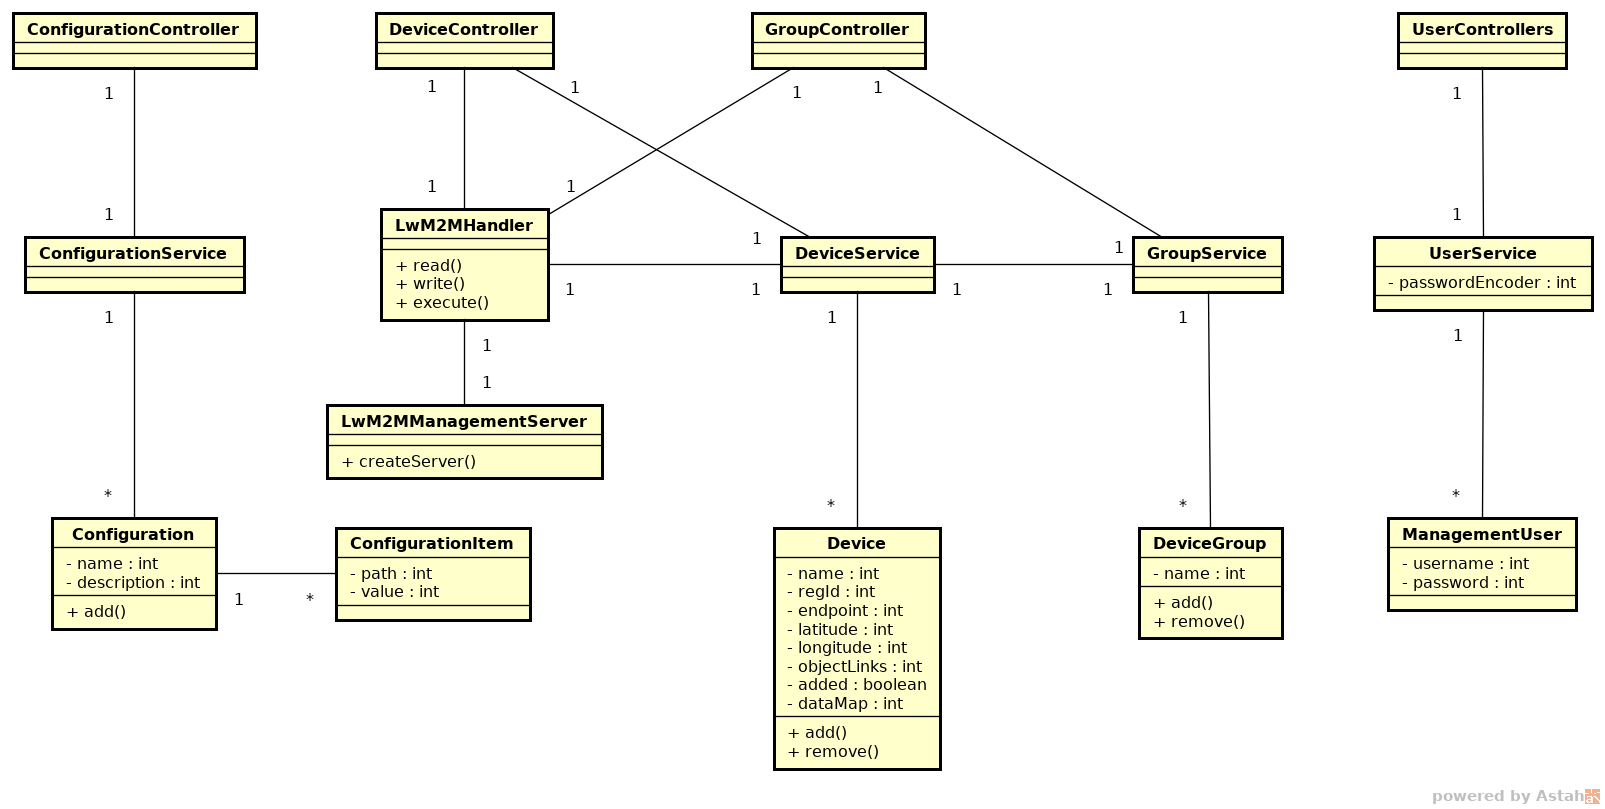
\includegraphics[width=1\textwidth]{images/domainmodel.png}
\caption{Klassendiagramm}
\end{figure}
\end{landscape}
\subsection{Klassenbeschreibungen}
\subsubsection{Connector}
Die Connector-Klasse ist für die Verbindung zu den Geräten zuständig. Sie behandelt die Authentisierung und stellt die Verbindung den anderen Klassen bereit. Dies ist eine zentrale Klassen, welche bei vielen Tätigkeiten benötigt wird.
\begin{table}[H]
\centering
    \begin{tabular}{@{}l p{14.1cm} @{}}\toprule    
    {Eigenschaft} & {Beschreibung}\\ \midrule
    connectToDevice() & Die Connect Methode, welche die Verbindung zu einem Device aufbaut. Bei der Verbindung wird dieser Klasse ein Device übergeben.\\
    \bottomrule
    \end{tabular}
\end{table}


\subsubsection{Discovery}
Dies ist die Discovery-Klasse. Mit der Discovery-Klasse wird auf Geräte aus dem Netzwerk gehört und falls welche vorhanden sind, werden diese in der Datenbank eingefügt. Für die verschiedenen Protokolle gibt es verschiedene Implementationen
\begin{table}[H]
\centering
    \begin{tabular}{@{}l p{14.1cm} @{}}\toprule    
    {Eigenschaft} & {Beschreibung}\\ \midrule
    listen() &  Die Methode wird beim Starten automatisch ausgeführt. Alle Anfragen werden verarbeitet und die neuen Geräte werden in der Datenbank abgelegt.\\
    \bottomrule
    \end{tabular}
\end{table}



\subsubsection{ConnectionHandler}
Mit dem ConnectionHandler werden die Daten von den Devices abgefragt, geschrieben, überwacht und ausgeführt. Je nach Device wird eine andere Implementation der Read-Funktion bereitgestellt, damit alle gewünschten Protokolle unterstützt werden.
\noindent \begin{table}[H]
\centering
    \begin{tabular}{@{}l p{14.1cm} @{}}\toprule    
    {Eigenschaft} & {Beschreibung}\\ \midrule      
    read() & Read-Methode, welche die Daten vom gewünschten Device ausliest.\\
    write() & Die write-Methode schickt die gewünschten Daten zum Device. \\
    \bottomrule
    \end{tabular}
\end{table}



\subsubsection{DeviceService}
Mit dem DeviceService wird eine Schnittstelle zum Data-Layer erstellt. Dieser Service ist für den kompletten Datenautausch zwischen den Schichten zuständig.\begin{table}[H]
\centering
    \begin{tabular}{@{}l p{14.1cm} @{}}\toprule    
    {Eigenschaft} & {Beschreibung}\\ \midrule 
    - & -
   \\ \bottomrule
    \end{tabular}
\end{table}




\subsubsection{FileHandler}
Der FileHandler ist für den Up- und Download zuständig. Er nimmt alle Dateien entgegen und speichert diese auf dem Server ab. Oder er holt eine Datei vom Server und lädt diese herunter, damit man sie mit dem Writer auf ein Device schicken kann.
\begin{table}[H]
\centering
    \begin{tabular}{@{}l p{14.1cm} @{}}\toprule    
    {Eigenschaft} & {Beschreibung}\\ \midrule 
    upload() & Mit dem Upload wird eine Datei vom Filesystem auf das Managementtool geladen. \\
    download() & Durch den download, kann eine Datei vom Managementtool heruntergeladen werden. \\
    \bottomrule
    \end{tabular}
\end{table}

\subsubsection{Device}
Device ist eine Datenklasse, welche alle Angaben eines Devices speichert. Jedes Device wird so in ein Objekt gespeichert.
\begin{table}[H]
\centering
    \begin{tabular}{@{}l p{14.1cm} @{}}\toprule    
    {Eigenschaft} & {Beschreibung}\\ \midrule      
    name & Gerätenamen \\
    protocolType & Protokolltyp, wie zum Beispiel CoAP, Http usw. \\
    authType & Authentifikationstyp wie zum Beispiel Passwort oder Zertifikat  \\
    entpoint & Endpunkt-Adresse des Gerätes \\
    credentials & Credentialobjekt, welches die Logindaten enthält
\\    \bottomrule
    \end{tabular}
\end{table}

\subsubsection{DeviceGroup}
Durch die DeviceGroup-Klasse wird das Composite-Pattern umgesetzt. So können die Geräte individuell verschachtelt werden.
\begin{table}[H]
\centering
    \begin{tabular}{@{}l p{14.1cm} @{}}\toprule    
    {Eigenschaft} & {Beschreibung}\\ \midrule      
    name & Device Gruppen Namen\\
    description & Beschreibung der Device Gruppe \\
    \bottomrule
    \end{tabular}
\end{table}

\subsubsection{Credential}
Credential-Klasse für die Devices. Durch diese Datenklasse werden alle Usernamen/Passwort kombinationen gehashed abgespeichert. Zusätzlich werden auch die jeweiligen Zertifikate hinterlegt.
\begin{table}[H]
\centering
    \begin{tabular}{@{}l p{14.1cm} @{}}\toprule    
    {Eigenschaft} & {Beschreibung}\\ \midrule      
    username & Benutzername des Devices \\
    password & Devicepassword als Hash\\
    certificate & Zertifikat als Datenblob\\
    hash() & Hashmethode, damit die Passwörter nicht im Klartext gespeichert werden\\
    \bottomrule
    \end{tabular}
\end{table}


\subsubsection{Command}
Mit der Command-Klasse werden alle benötigten Kommandos, wie zum Beispiel "Shutdown" usw. erfasst.
\begin{table}[H]
\centering
    \begin{tabular}{@{}l p{14.1cm} @{}}\toprule    
    {Eigenschaft} & {Beschreibung}\\ \midrule      
    command & Device-Kommando\\
    \bottomrule
    \end{tabular}
\end{table}


\subsubsection{File}
Das Interface File, bestimmt die Methoden und Variablen, welche die Vererbten Klassen implementieren müssen.
\begin{table}[H]
\centering
    \begin{tabular}{@{}l p{14.1cm} @{}}\toprule    
    {Eigenschaft} & {Beschreibung}\\ \midrule      
    name & Name der abgelegten Datei\\
    date & Datum\\ 
    Version & Versionsstand der Software oder der Konfigurationsdatei\\
    \bottomrule
    \end{tabular}
\end{table}


\subsubsection{ConfigFile}
Die ConfigFile-Klasse ist die Datenklasse für alle Konfigurationsdateien, damit diese in einer Datenbank angepassten Form gespeichert werden können. \begin{table}[H]
\centering
    \begin{tabular}{@{}l p{14.1cm} @{}}\toprule    
    {Eigenschaft} & {Beschreibung}\\ \midrule      
    - & -\\
    \bottomrule
    \end{tabular}
\end{table}



\subsubsection{SoftwareFile}
Diese Datenklasse ist das Objekt für eine Softwaredatei. So kann die Datei in der Datenbank erfasst werden.
\begin{table}[H]
\centering
    \begin{tabular}{@{}l p{14.1cm} @{}}\toprule    
    {Eigenschaft} & {Beschreibung}\\ \midrule      
    - & -\\
    \bottomrule
    \end{tabular}
\end{table}



\subsubsection{CertificateFile}
Zertifikatdatei-Datenklasse. Mit dieser Klasse werden Zertifikate in Objekte umgewandelt, damit man sie in der Datenbank abspeichern kann.
\begin{table}[H]
\centering
    \begin{tabular}{@{}l p{14.1cm} @{}}\toprule    
    {Eigenschaft} & {Beschreibung}\\ \midrule      
    - & -\\
    \bottomrule
    \end{tabular}
\end{table}


\section{Logische Architektur}
\begin{figure} [H]
	\begin{center}
	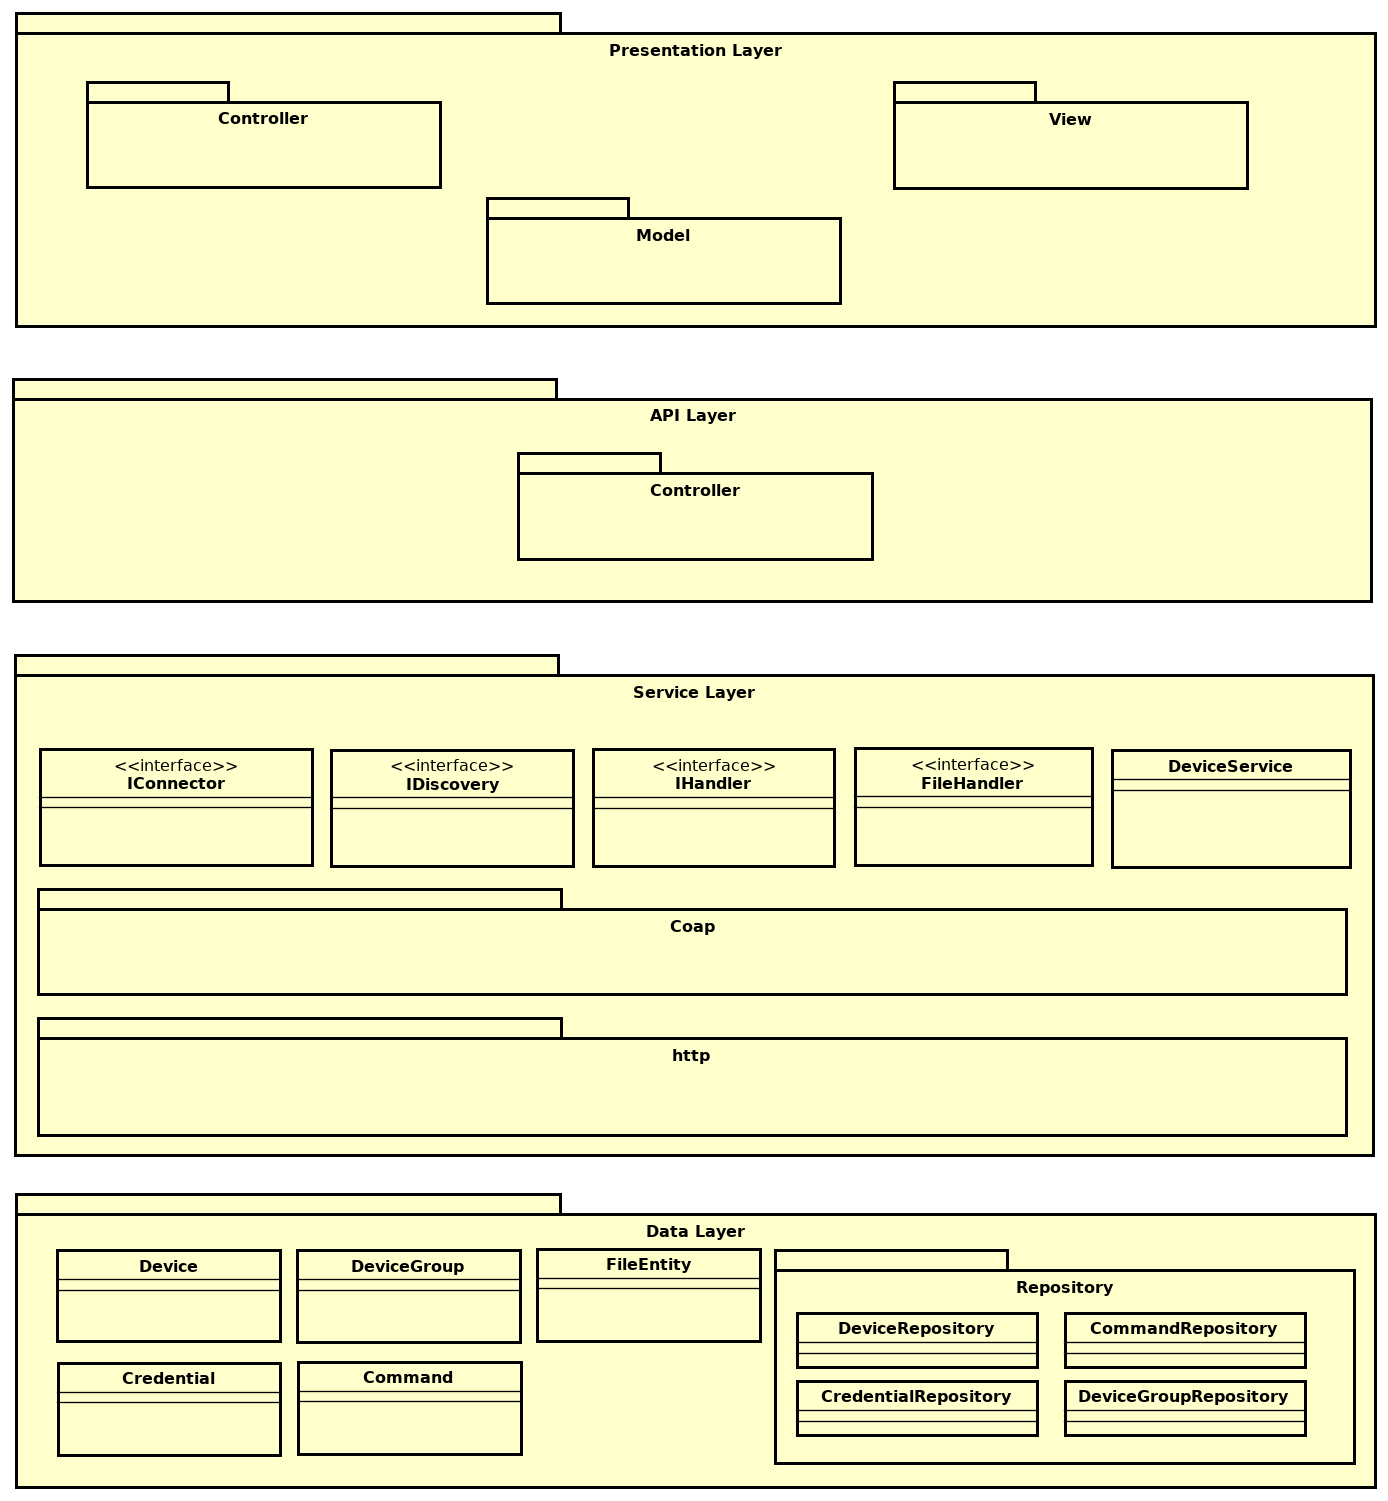
\includegraphics[width=0.90\textwidth]{images/architektur.png}
	\caption{Logische Architektur}
	\end{center}
\end{figure}


\subsection{Presentation Layer}
Im Presentation-Layer wird das MVC-Pattern umsetzt. Dazu wird ein Controller, eine View sowie ein Model Package implementiert, welche alle Anfragen bearbeiten und anzeigen. Der Presentation-Layer liegt komplett auf der Clientseite.
\subsubsection{Packagestruktur}
\begin{table}[H]
\centering
    \begin{tabular}{@{}l p{14.1cm} @{}}\toprule    
    {Packagename} & {Beschreibung}\\ \midrule
    Controller & Der Controller verwaltet alle Anfragen der View und bearbeitet das Model dementsprechend.\\       
    View & Die View bekommt von dem Model die Daten und Renderd dazu die jeweiligen Anzeigen. \\
    Model & Im Model werden alle Daten gehalten, welche die View anzeigt. Nur der Controller hat direkten Zugriff auf diese Daten. \\
    \bottomrule
    \end{tabular}
\end{table}
\subsubsection{Schnittstellen}
Der Presentation-Layer liegt separat auf dem Client, daher gibt es nur eine Schnittstelle über die Rest API auf den Server. Über dieses API werden alle Daten geholt und auf dem Client gerendert und angezeigt.



\subsection{API Layer}
Der oberste Layer auf der Backend Seite ist der API Layer. Dieser bietet alle wichtigen Schnittstellen an und bearbeitet die Anfragen. Dazu werden in den Controller Klassen die RequestMappings erstellt. Die Anfragen werden an den Service Layer gegeben, welche die Applikation Logik beinhaltet.
\subsubsection{Packagestruktur}
\begin{table}[H]
\centering
    \begin{tabular}{@{}l p{14.1cm} @{}}\toprule    
    {Packagename} & {Beschreibung}\\ \midrule
    Controller & Der Controller verwaltet alle Anfragen vom dem Client Frontend und verarbeitet diese.\\       
    \bottomrule
    \end{tabular}
\end{table}
\subsubsection{Schnittstellen}
Der API Layer hat eine direkte Schnittstelle zum Service Layer. Alle Anfragen werden über diese Schnittstelle verarbeitet, damit das API sauber von der Datenverarbeitung getrennt ist. 


\subsection{Service-Layer}
Der Service-Layer beinhaltet die Backend Klassen, welche für die Verarbeitung der Daten zuständig ist. Hier werden alle Devices erfasst, verbunden und verwaltet. Dazu wird jedes gefundene Device auf der Datenbank hinterlegt. Bei einem Read und Write wird das Device aus dem Data Layer geholt und mit den neuen Daten aktualisiert.
\subsubsection{Klassenstruktur}
\begin{table}[H]
\centering
    \begin{tabular}{@{}l p{14.1cm} @{}}\toprule    
    {Klassenname} & {Beschreibung}\\ \midrule
     IConnector & Die Verbindungsklasse des Servicelayer stellt alle Verbindungen zu den Devices auf.  \\       
     IDiscovery & Der Listener horcht auf neue Devices und erfasst diese laufend auf dem Data-Layer  \\       
     IHandler &  Der IHandler ist für die Read, Write, Observe und Execute Befehle zuständig.\\       
     FileHandler &   Liest und schreibt alle File Objekte\\       
     DeviceService &  Schnittstelle zum Data Layer. Liest und schreibt alle Device Objekte \\       
    \bottomrule
    \end{tabular}
\end{table}
\subsubsection{Schnittstellen}
Der Service-Layer hat eine Schnittstelle zum Data-Layer. Durch den Service-Layer werden die Datenobjekte erstellt, bearbeitet und ausgewertet. Der API Layer muss immer über den Service-Layer, um eine saubere Abtrennung der Schichten zu gewährleisten.

\subsection{Data-Layer}
Der Data-Layer beinhaltet alle Datenobjekte, welche vom laufenden Programm benötigt werden. Diese werden von hier in die Datenbank geschrieben. Das Repository bietet die Datenbankmethoden an, um die Daten in die Datenbank zu speichern.
\subsubsection{Klassenstruktur}
\begin{table}[H]
\centering
    \begin{tabular}{@{}l p{14.1cm} @{}}\toprule    
    {Klassenname} & {Beschreibung}\\ \midrule
    Device & Device ist eine Datenklasse, welche alle Daten von einem Device beinhaltet.\\
    Credentials & Alle Zugriffsdaten der Devices sind in der Credentials-Klasse definiert. \\
    DeviceGroup & In der Datenklasse DeviceGroup, werden alle Gruppen verwaltet, damit das Composite-Pattern umgesetzt werden kann.\\
    Command & Alle Kommandos werden zentral in der Command-Datenklasse gespeichert.\\
    FileEntitiy & In FileEntitiy wird das Grundgerüst für alle Dateien erstellt, damit diese in einer geeigneten Form in der Datenbank abgespeichert werden können.\\    
    Repository & Schnittstelle zur Datenbank. Bietet die Datenbankmethonden, wie Insert, Delete, Find usw. an.\\     
    \bottomrule
    \end{tabular}
\end{table}
\subsubsection{Schnittstellen}
Da der Data Layer die unterste Schicht ist, gibt es nur eine Verbindung zur Datenbank.